Design in power electronics—encompassing topology selection, parameter tuning, and reliability assurance—often involves high-dimensional, nonlinear optimization problems, further complicated by tight constraints. Traditional design workflows—relying on expert experience, manual iterations, and slow simulations—typically lead to suboptimal convergence and prolonged design cycles. This is particularly evident 

\begin{figure}[htbp]
    \centering
    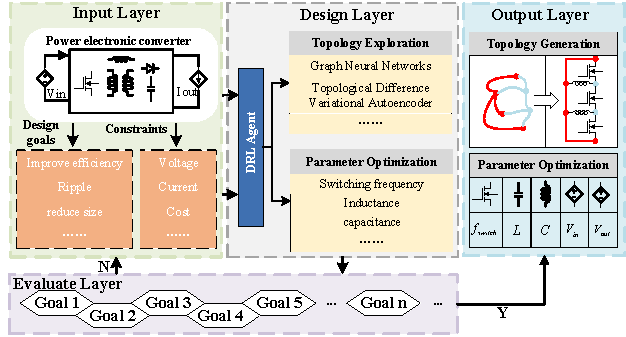
\includegraphics[width=\linewidth]{fig/design_overview.pdf}
    \caption{Flowchart of DRL design for power electronic converters.}
    \label{fig:topo_overview}
\end{figure}

\noindent in topology discovery and component coordination, where conventional methods struggle with efficiency and adaptability.

Recent advancements in AI, particularly DRL, offer promising solutions to these challenges. DRL introduces a data-driven approach capable of autonomously learning design strategies by interacting with its environment. Unlike traditional heuristic-based optimization methods, DRL enables adaptive exploration of complex design spaces, effectively handling sparse rewards and multi-objective trade-offs. This adaptability makes DRL particularly well-suited for optimizing two critical sub-tasks in PEC design: topology exploration and parameter optimization. Fig.~\ref{fig:topo_overview} presents a systematic flowchart of DRL design in PECs.

\subsection{Topology Exploration}
\label{sec:topo_explore}

Recent advances in topology exploration for PECs have been achieved through the integration of artificial intelligence, particularly RL and graph-based models. Approaches can be broadly classified into three categories: adjacency-matrix-driven methods, graph-based learning frameworks, and hybrid generative models.

Adjacency-matrix-driven strategies, such as the method proposed by Chen et al.~\cite{9615058}, leverage neural networks within a Q-learning paradigm to iteratively build converter topologies. As illustrated in Fig.\ref{fig:chen_framework}, the state of the system is encoded as a custom adjacency matrix that reflects component interconnections. The RL agent employs Q-learning to progressively construct the circuit, with its policy refined through reward functions based on electrical feasibility, loop extraction, and voltage-second balance. This method achieves fully automatic topology deduction without requiring expert knowledge or prior feature engineering, effectively balancing forward and reverse design processes to discover both known and novel topologies.

\begin{figure}[t]
    \centering
    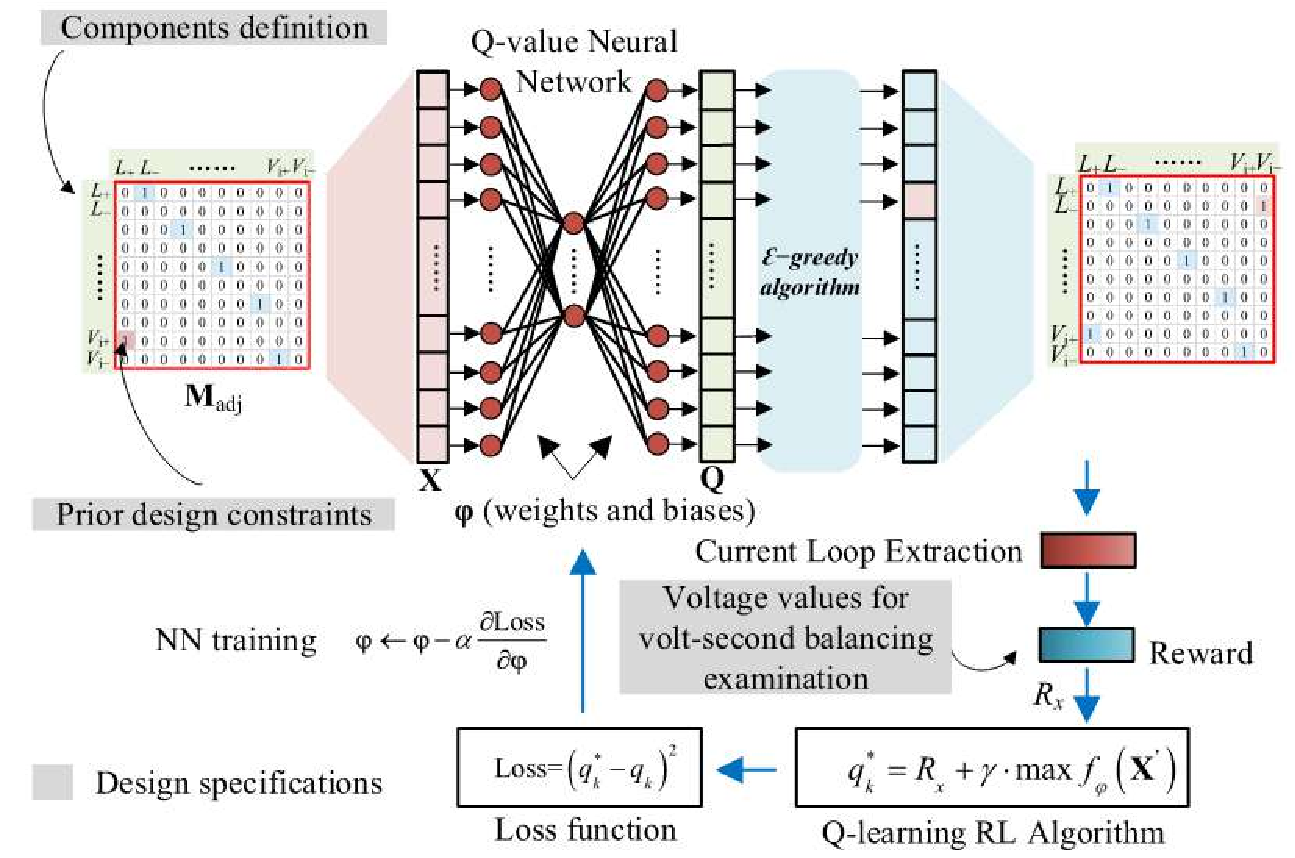
\includegraphics[width=0.9\linewidth]{fig/chen_framework.pdf}
    \caption{Architecture of the RL-based topology deduction method by Chen et al.~\cite{9615058}.}
    \label{fig:chen_framework}
\end{figure}

Beyond adjacency-matrix encoding, a nonisolated single-inductor multiport (SIMP) DC-DC topology deduction framework has been proposed in \cite{chen2021nonisolated}, which integrates forward and reverse design principles within a reinforcement learning paradigm. Specifically, a neural network is employed to conduct forward design by predicting feasible connection patterns, while a rule-based reward function guides reverse design to ensure electrical validity and performance compliance. Unlike conventional feature engineering or exhaustive combinatorial search, this approach only requires basic design specifications (e.g., component availability and port voltage levels) as inputs, thereby lowering the knowledge barrier for non-expert designers. Through iterative trial-and-error interactions, the RL agent accumulates experience and progressively constructs topologies that maximize the defined reward. This method not only successfully rediscovered a wide range of SIMP converter topologies reported in the literature but also generated novel architectures, one of which was experimentally validated to confirm its practical feasibility. Compared to adjacency-matrix-driven methods, the SIMP framework emphasizes interpretability and accessibility, providing a complementary pathway for automatic topology exploration with reduced implementation complexity.

In contrast, graph-based deep learning approaches~\cite{liang2022learning,10012061} model circuits as undirected graphs and employ Graph Neural Networks (GNNs) in conjunction with actor-critic RL algorithms, notably PPO. Specifically, Liang et al.~\cite{liang2022learning} introduced a GNN-driven framework that extracts high-level features from circuit graphs, enabling the agent to sequentially attach new functional blocks and efficiently explore the vast topology space. This method dramatically reduces the computational burden, scaling the time to find feasible circuits from exponential to near-linear and achieving over 30\% reduction in switch count compared to conventional combinatorial search methods. Experimental validation confirms stable converter outputs and strong adherence to circuit constraints. Extending this paradigm, Dong et al.\cite{10012061} further integrated advanced constraint management into the PPO-GNN framework, as depicted in Fig.\ref{fig:dong_framework}. Their approach ensures generated topologies meet both hard (electrical) and soft (performance) constraints, such as voltage and current stresses. As a result, the generation time for complex 8-port converter topologies was reduced by an order of magnitude, with derived circuits demonstrating 50\% lower voltage stress and 31\% lower current stress relative to baseline designs. These results underscore the capacity of DRL-empowered frameworks to rapidly discover and optimize sophisticated multiport converter topologies, marking a substantial leap in both efficiency and circuit quality.
\begin{figure}[t]
    \centering
    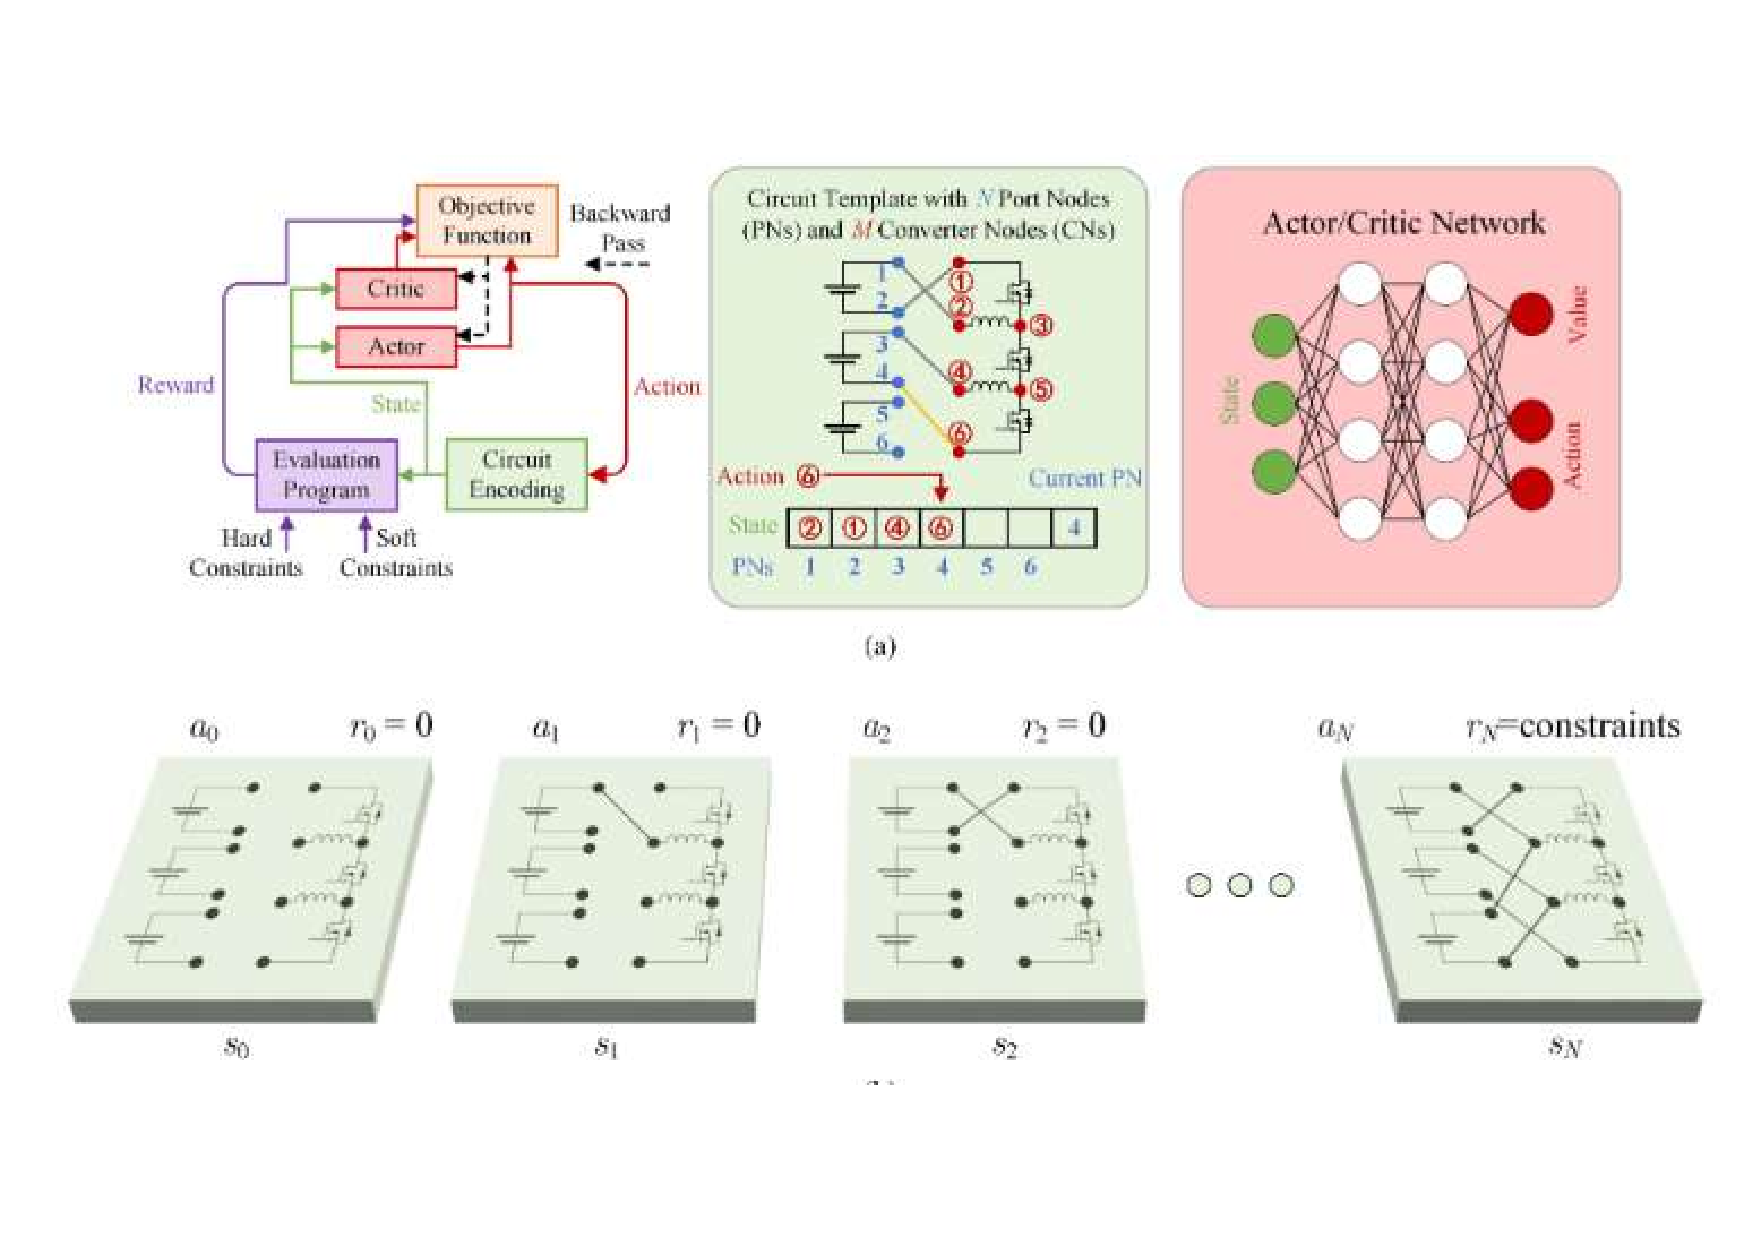
\includegraphics[width=0.9\linewidth]{fig/dong_framework.pdf}
    \caption{RL-PPO-based automated topology generation framework by Dong et al.~\cite{10012061}.}
    \label{fig:dong_framework}
\end{figure}

More recently, hybrid generative frameworks have emerged, combining variational autoencoder (VAE)-based models with reinforcement learning to further enhance the diversity and controllability of topology generation. Xu et al.~\cite{xu2022power} proposed a novel method leveraging the TopoDiffVAE—a topological difference variational autoencoder—integrated with RL for converter topology derivation. As shown in Fig.\ref{fig:topodiffvae_framework}, TopoDiffVAE is first trained on a dataset of graph-represented converter topologies to learn implicit structural features. The decoder 

\begin{figure}[t]
    \centering
    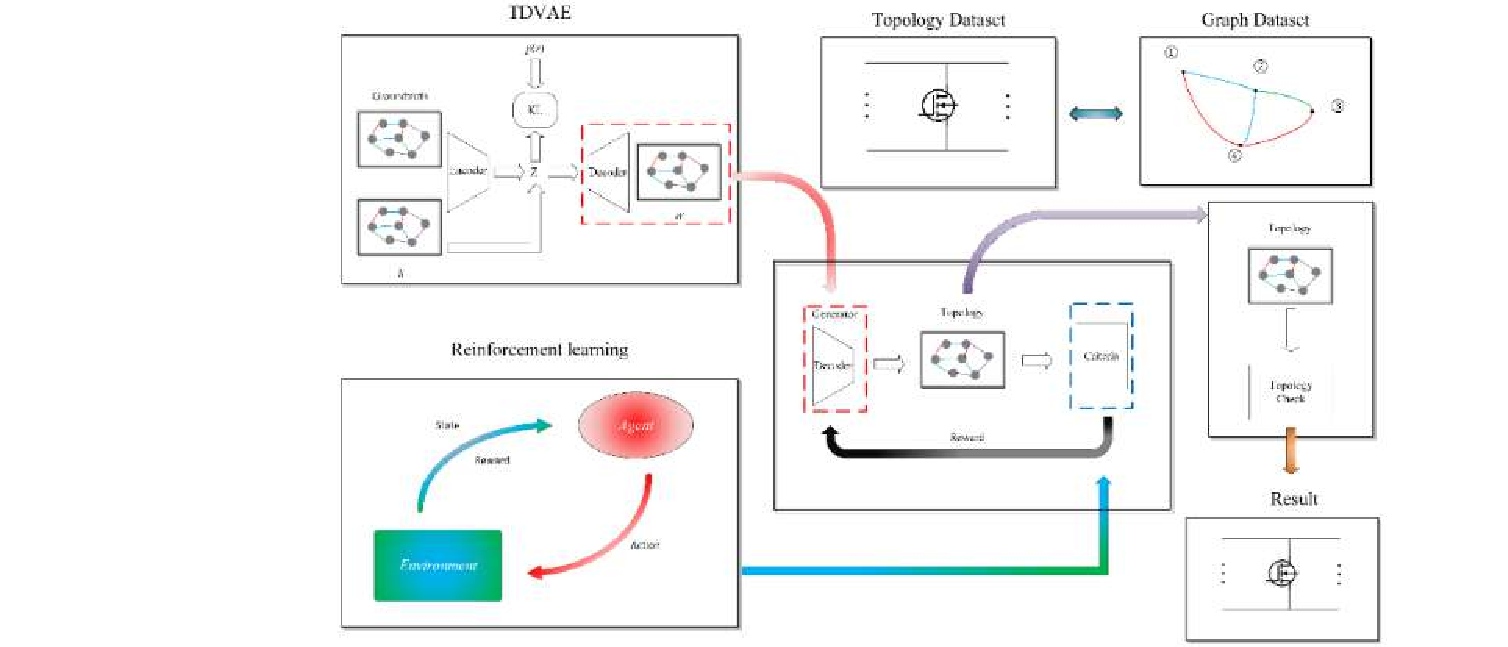
\includegraphics[width=0.9\linewidth]{fig/topodiffvae_framework.pdf}
    \caption{Architecture of the TopoDiffVAE and RL-based topology generation framework by Xu et al.~\cite{xu2022power}.}
    \label{fig:topodiffvae_framework}
\end{figure}

\begin{table*}[htbp]
\centering
\caption{Summary of Topology Exploration in Power Electronics Converters Using DRL}
\label{tab:Topology_Exploration}
\resizebox{\textwidth}{!}{
\begin{tabular}{@{}c p{2.5cm} c p{4.5cm} p{5cm}@{}}
\toprule
\textbf{Reference} & \textbf{Topology} & \textbf{Algorithm} & \textbf{Features} & \textbf{Advantages \& Disadvantages} \\ 
\midrule
\cite{9615058} & Non-isolated SIMP DC-DC Converters & QL & 
- Efficient topology exploration \newline
- No expert knowledge required \newline
- Focus on multiport converters & 
\textbf{Advantage:} \newline
- Heterogeneous topology generation \newline
- Low implementation complexity \newline
\textbf{Disadvantage:} \newline
- No hardware implementation \newline
- Post-processing needed to exclude equivalent topologies \newline
- Linear complexity growth \\ \midrule

\cite{liang2022learning} & Multiport DC-DC Converters & PPO & 
- Multiport DC-DC topology derivation \newline
- Incorporates hard and soft constraints \newline
- Optimizes voltage and current stresses & 
\textbf{Advantage:} \newline
- Reduced time complexity \newline
- Improved topology quality \newline
- Effective performance optimization \newline
\textbf{Disadvantage:} \newline
- Requires careful constraint definition \newline
- Complex for real-world applications \\ \midrule

\cite{10012061} & Multiport DC-DC Converters & AC \& GNNs & 
- GNN extracts features \newline
- DRL constructs topology step-by-step with constraints & 
\textbf{Advantage:} \newline
- Flexible topology generation \newline
- Handles complex circuits \newline
\textbf{Disadvantage:} \newline
- High computational cost \newline
- Challenging to implement on hardware \\ \midrule

\cite{xu2022power} & General PECs Topologies & TopoDiffVAE \& RL & 
- Combines TopoDiffVAE with DRL for faster topology generation & 
\textbf{Advantage:} \newline
- Fast and accurate \newline
\textbf{Disadvantage:} \newline
- Requires large dataset for training \newline
- Complex hardware deployment \\ 
\bottomrule
\end{tabular}
}
\end{table*}



\noindent
then serves as a topology generator within a reinforcement learning loop, where explicit circuit constraints (e.g., short-circuit prevention, component count, and forbidden series connections) are enforced through reward shaping. Unlike traditional RL, this approach allows the agent to evaluate entire candidate topologies, guiding the generative process to produce valid and novel converter configurations, including those not present in the original training set. Experimental results confirm that this hybrid method accelerates topology generation and improves accuracy compared to purely data-driven approaches, representing a promising direction for integrating deep generative modeling with RL-based constraint optimization in power electronics topology exploration.

Collectively, these studies establish that the combination of RL, GNNs, generative models, and structured circuit encoding offers a scalable and automated pathway for topology exploration, outperforming traditional rule-based or exhaustive search strategies. The integration of domain-specific reward shaping and constraint management is crucial for ensuring practical feasibility, while the modular nature of these frameworks enables future adaptation to diverse converter architectures and operating conditions. The summary of selected DRL algorithm for topology exploration is shown in Table~\ref{tab:Topology_Exploration}.


\subsection{Parameter Optimization}
\label{sec:param_opt}

The optimization of design parameters in PECs is crucial to improving efficiency, power density, thermal performance, and overall cost-effectiveness. Recent advancements in DRL have offered powerful tools to automate this optimization process, overcoming the limitations of traditional design methods, which often rely on manual adjustments and trial-and-error. DRL enables faster and more accurate parameter adjustments, significantly enhancing design flexibility and performance optimization under varying conditions.

Recent studies have demonstrated the effectiveness of DRL in optimizing various parameters across different components of PECs. For example, Tian et al. \cite{tian2022deep, tian2022parameter} applied the DDPG algorithm to optimize the design of a DC-DC synchronous buck converter. The focus of their work was on optimizing the inductor design by adjusting parameters such as the number of turns, air gap size, and core material. This optimization led to a 4.5\% reduction in power losses, showing that DRL can significantly enhance inductor design efficiency and reduce energy losses. Fig.~\ref{fig:tian2022} shows the schematic of the optimized DC-DC synchronous buck converter. Building on this, Tian et al. \cite{tian2024optimizing} extended their work to DC inductors with air gaps, addressing thermal stress optimization alongside electrical performance. The use of DDPG resulted in an 11.91\% reduction in thermal stress, maintaining high electrical performance and improving the converter's overall reliability and longevity.

\begin{figure}[htbp]
    \centering
    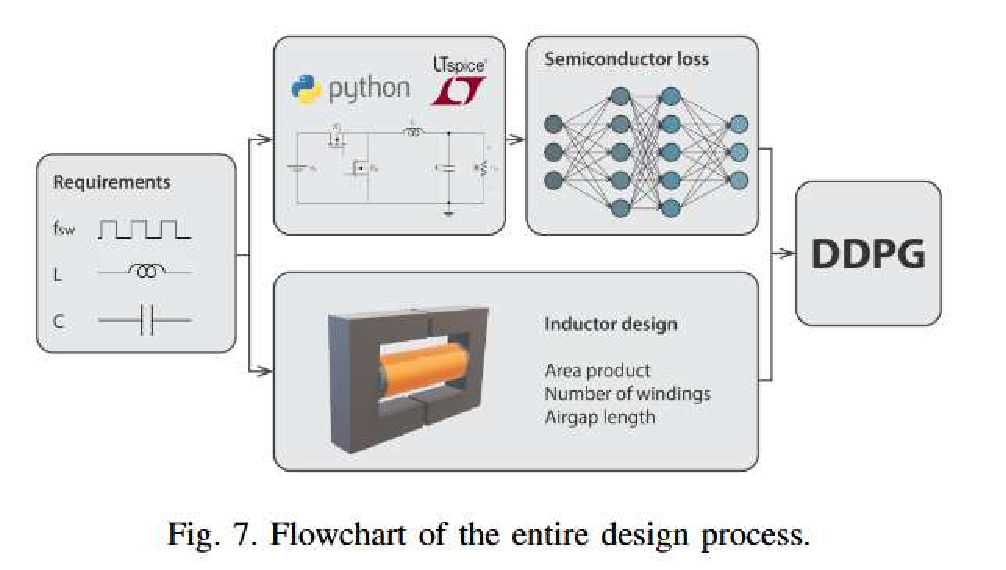
\includegraphics[width=0.9\linewidth]{fig/design5.pdf} 
    \caption{Optimized DC-DC synchronous buck converter design by Tian et al.~\cite{tian2022deep}.}
    \label{fig:tian2022}
\end{figure}

In parallel, Bui et al. \cite{bui2022deep} proposed a DRL-based surrogate model for optimizing the component sizing of power converters. By combining DNN to model semiconductor losses and DRL to optimize parameters such as capacitance, inductance, and switching frequency, their approach achieved a 6.3\% increase in power efficiency. The integration of SAC ensured the system avoided local optima, handling large state and action spaces effectively. This was further extended by Bui et al. \cite{bui2023deep}, who used PPO to optimize multi-objective parameters such as power efficiency and size for Buck and Boost converters. Their results showed a significant improvement in power efficiency from 94.5\% to 97.7\%, while reducing the converter size by 5\%, demonstrating DRL's capability in multi-objective optimization tasks. Fig.~\ref{fig:bui2022} displays the DRL-based surrogate model for optimizing power converter components.

\begin{figure}[htbp]
    \centering
    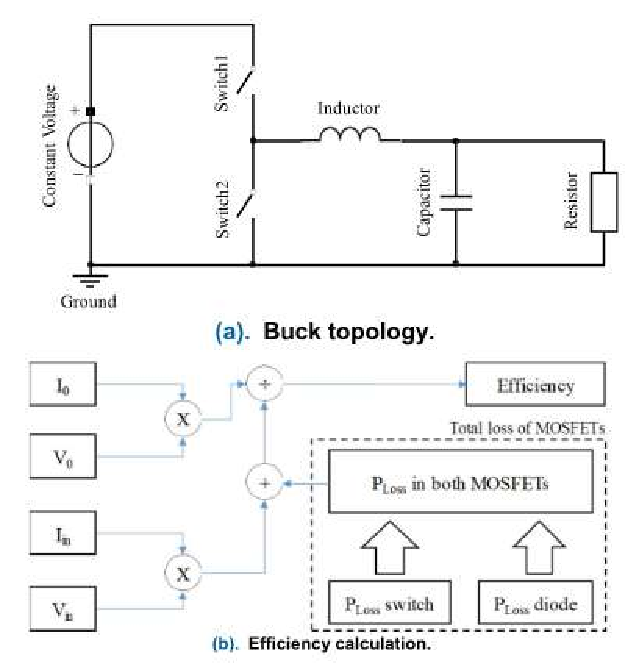
\includegraphics[width=0.9\linewidth]{fig/design6.pdf} 
    \caption{DRL-based surrogate model for power converter component optimization by Bui et al.~\cite{bui2022deep}.}
    \label{fig:bui2022}
\end{figure}

Moreover, Wang et al. \cite{wang2022efficiency, wang2023efficiency, wang2024case, wang2023modeling} explored DRL applications in the optimization of three-level inverters, with a focus on efficiency and power density. By applying DDPG, they optimized parameters such as switching frequency and modulation index, resulting in a 5.3\% improvement in efficiency and a 7.5\% increase in power density. These findings demonstrate DRL’s potential in optimizing high-power systems, balancing both performance and compactness, which are essential for modern power electronics applications. Fig.~\ref{fig:wang2025} showcases the optimized three-level inverter system.

\begin{figure}[htbp]
    \centering
    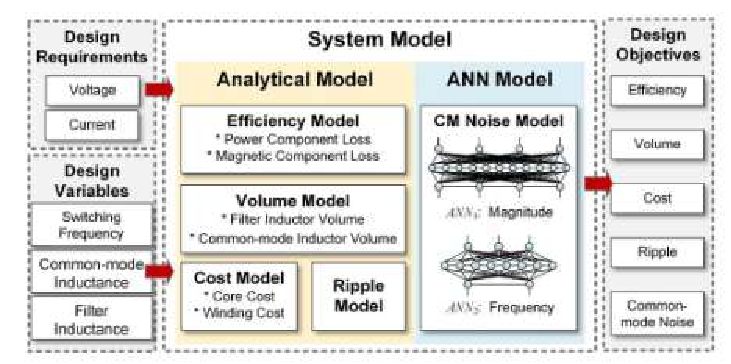
\includegraphics[width=0.9\linewidth]{fig/design7.pdf} 
    \caption{Optimized three-level inverter design by Wang et al.~\cite{wang2024case}.}
    \label{fig:wang2025}
\end{figure}

These studies collectively highlight the versatile role of DRL in optimizing PEC parameters. From DC-DC converters to multi-objective optimization in resonant converters and inverters, DRL has demonstrated its ability to improve critical design parameters, such as efficiency, power density, and thermal stress, across various components of PECs. By enabling faster, more accurate parameter adjustments and offering solutions for multi-objective optimization, DRL provides substantial advantages over traditional design methods. The summary of selected DRL algorithm for parameter optimization is shown in Table~\ref{tab:parameter_optimization_summary}.

%\subsection{Discussion}
%\label{sec:design_conclusion}

%In conclusion, DRL has demonstrated its transformative potential in the design and optimization of PECs, particularly in the automation of topology exploration and parameter optimization. DRL techniques, such as PPO, DDPG, and SAC, have shown remarkable success in improving efficiency, reducing losses, and accelerating the design process, making them essential tools for modern PECs. The ability of DRL to handle complex, multi-objective optimization tasks allows for faster and more precise designs, offering significant advancements over traditional optimization methods. However, there are several challenges that remain. While DRL methods excel in specific applications, they still face issues such as high computational cost, limited scalability to large systems, and challenges related to sparse rewards during training. Additionally, there is a need for further research into enhancing the robustness and generalizability of these algorithms across diverse power electronic systems. Moreover, integrating DRL with traditional methods in a hybrid approach could help leverage the strengths of both techniques, ensuring the reliability and performance of PEC designs in real-world applications. Future work should focus on addressing these limitations, improving the adaptability of DRL to more complex, large-scale systems, and exploring its integration with domain-specific knowledge to achieve more interpretable and physically grounded solutions.
\begin{table*}[htbp]
\centering
\caption{Summary of Parameter Optimization in PECs Using DRL}
\label{tab:parameter_optimization_summary}
\renewcommand{\arraystretch}{1.3}
\begin{tabular*}{\textwidth}{@{\extracolsep{\fill}} c p{2.5cm} c p{4.5cm} p{6cm} @{}}
\toprule
\textbf{Reference} & \textbf{Problem Optimized} & \textbf{Algorithm} & \textbf{Parameters Optimized} & \textbf{Features} \\ 
\midrule
\cite{tian2022deep} & DC-DC converter parameter optimization & DQN & 
\textbf{Inductor design:} \newline
- Turns \newline
- Air gap \newline
- Core material & Enhancing efficiency by selecting the optimal design based on performance simulations. \\ 
\midrule
\cite{tian2022parameter} & Parameter optimization for DC-DC power converters & DDPG & 
- Semiconductor losses \newline
- Magnetic design parameters & Combined DDPG with ANNs to optimize semiconductor losses and magnetic design. \\ 
\midrule
\cite{tian2024optimizing} & DC inductor design optimization & DDPG & 
\textbf{Inductor design:} \newline
- Air gap \newline
- Winding turns \newline
- Core material & Integrated thermal stress and electrical optimization. \\ 
\midrule
\cite{bui2022deep} & Optimal component sizing for power converters & SAC & 
\textbf{Converter parameters:}  \newline
- Inductors \newline
- Capacitors \newline
- Switching frequency & Integrated DRL with a deep neural network-based surrogate model. \\ 
\midrule
\cite{bui2023deep} & Optimal parameter design of power converters & PPO & 
- Switching frequency \newline
- Inductance \newline
- Capacitance & Multi-objective design optimization; emphasizing stability, faster convergence, and efficient control. \\ 
\midrule
\cite{wang2022efficiency} & Efficiency optimization of Three-level ANPC Inverter & DDPG & 
- Efficiency \newline
- Power loss & Demonstrated DRL’s ability to handle complex power converter design tasks in real-world applications. \\ 
\midrule
\cite{wang2023efficiency} & Efficiency and power density optimization for LLC Resonant Converter & DDPG & 
- Switching frequency \newline
- Power loss \newline
- Volume & Optimized both efficiency and power density; addressing challenges of power conversion and compact system design. \\ 
\midrule
\cite{wang2024case} & Multi-objective optimization of ANPC Inverter & DDPG & 
- Switching frequency \newline
- Component volume \newline
- Current ripple \newline
- Cost & Combined DRL with traditional engineering heuristics; optimizing efficiency, size, and cost simultaneously. \\ 
\midrule
\cite{wang2023modeling} & TSV inductor design in on-chip DC-DC converters & DDPG & 
- Inductor geometry \newline
- Thermal stress \newline
- Parasitic capacitance & Introduced thermal-stress-coupled optimization with DRL; balancing thermal stress reduction with electromagnetic performance. \\
\bottomrule
\end{tabular*}
\end{table*}


